% !TEX root=../thesis.tex

%	Is information about details 
%	unnecessary for progression of the reading put into appendixes? 


\chapter{Results}
\label{chapter:results}

In this chapter we present the results from our research and architecture design efforts. We also present a top-level view of the systems hardware
architecture, some of which have been defined by our findings, and some which
comes from the need to integrate with other hardware on our technical testbed -
Revolve's 2014 car. 

\section{Stakeholders}
\label{results:stakeholders}
During analysis and workshops we defined the three main stakeholders;
developers, Revolve, and drivers. Since the FS competitions' business case
involves trying to sell the vehicle as a product to be mass manufactured for
racing purposes we elected to adopt some fictional stakeholders to get a full
picture of who the system is supposed to cater to. These stakeholders are
non-professional drivers and vehicle owners who for instance rents out cars. We
also considered the potential that somebody would want to implement the system
in their car and what they would need to do to interface with the system.

\section{Hardware}
In our research we found that the traditional dashboard does not fare well in
its task of communicating information during racing or practice (see \vref{interview:bakkom}).
The pace during racing does not allow for spending time looking at the
instruments, and therefore the most effective way of conveying information is
through flashing lamps which can be picked up by the drivers peripheral vision
(also see Chen et al. \cite{cheng2007intelligentVehicles} who supports this 
point in their 2007 study).
This is further supported by findings in other studies; when drivers are
distracted, either cognitively, visually, or with activities, their response
times increase and the likelihood of accidents increase \cite{hancock1999effects,visualDistractionsStudy}.
Other studies find that using head-up displays reduce both cognitive workload, give better reaction times, and increases the time spent looking at the
road
\cite{BMW,huang2013effects,Liu:HudPerformance,nishizawa1997heads,cheng2007intelligentVehicles,lim1999heads}.

\label{results:wearableHud}
Placing a HUD in a vehicle can be done in many ways. Ordinary cars have theirs
placed in the dashboard, putting the display on the windshield. However,
studies of video footage show that having a fixed position HUD in a FSAE-car
would provide little improvement over the dashboard. First, there is no windshield,
and second the driver spend a lot of time with the head turned to the sides.

Our proposed system design is therefore to utilize a wearable display 
device to put a HUD in front of the driver's eye(s). This imposes
one important restriction: The system cannot hinder the drivers egress from
the vehicle, see article 4.8 \cite{fsae:2014rules}. According to the rules the
driver must be able to exit the vehicle from a fully seated driving position in
no more than 5 seconds. Therefore our proposal is that the HUD system should
utilize wireless communication to get a data feed from the vehicle during operation (see \ref{fig:simple-hw}), and operate off battery power.
That way, no wires will be in the way and the driver can move freely in and out
of the vehicle. 
\begin{figure}[!htbp]
	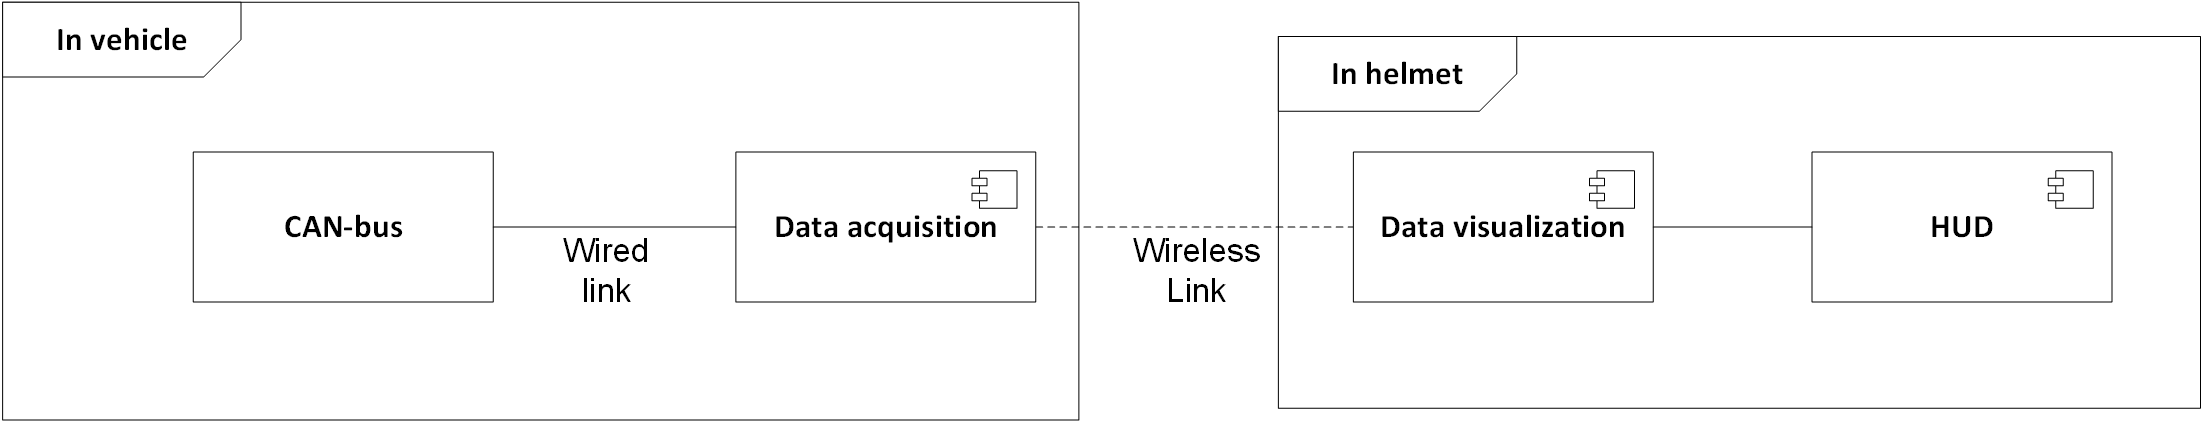
\includegraphics[width=\textwidth]{simple-hw-arch.png}
	\caption{Simple block-diagram of our proposed hardware architecture.}
	\label{fig:simple-hw}
\end{figure}

\section{Requirements and Software Architecture}
Since the system to be developed includes both hardware and software the
requirements covers aspects of both, but most of the hardware architecture is
defined by the vehicle that it is to be fitted to and, the rest is defined by
the decision to use a wearable HUD-device.

Some of the most architecturally important requirements are the following:
\begin{itemize}
\item Rapid configuration of display layout.
\item Ability to create a sensor calibration profile without compilation of
code.
\item Rapid configuration of sensor profiles, including package data format. 
\item Display of real-time data.
\end{itemize}
For the complete system requirements and system architecture factors we refer to the following appendices: Vision document \vref{appendix:vision},
requirements document \vref{appendix:requirements}, supplementary specification
document
\vref{appendix:supspec}, and the system architecture document \vref{appendix:sad}.

\begin{figure}[!htbp]
	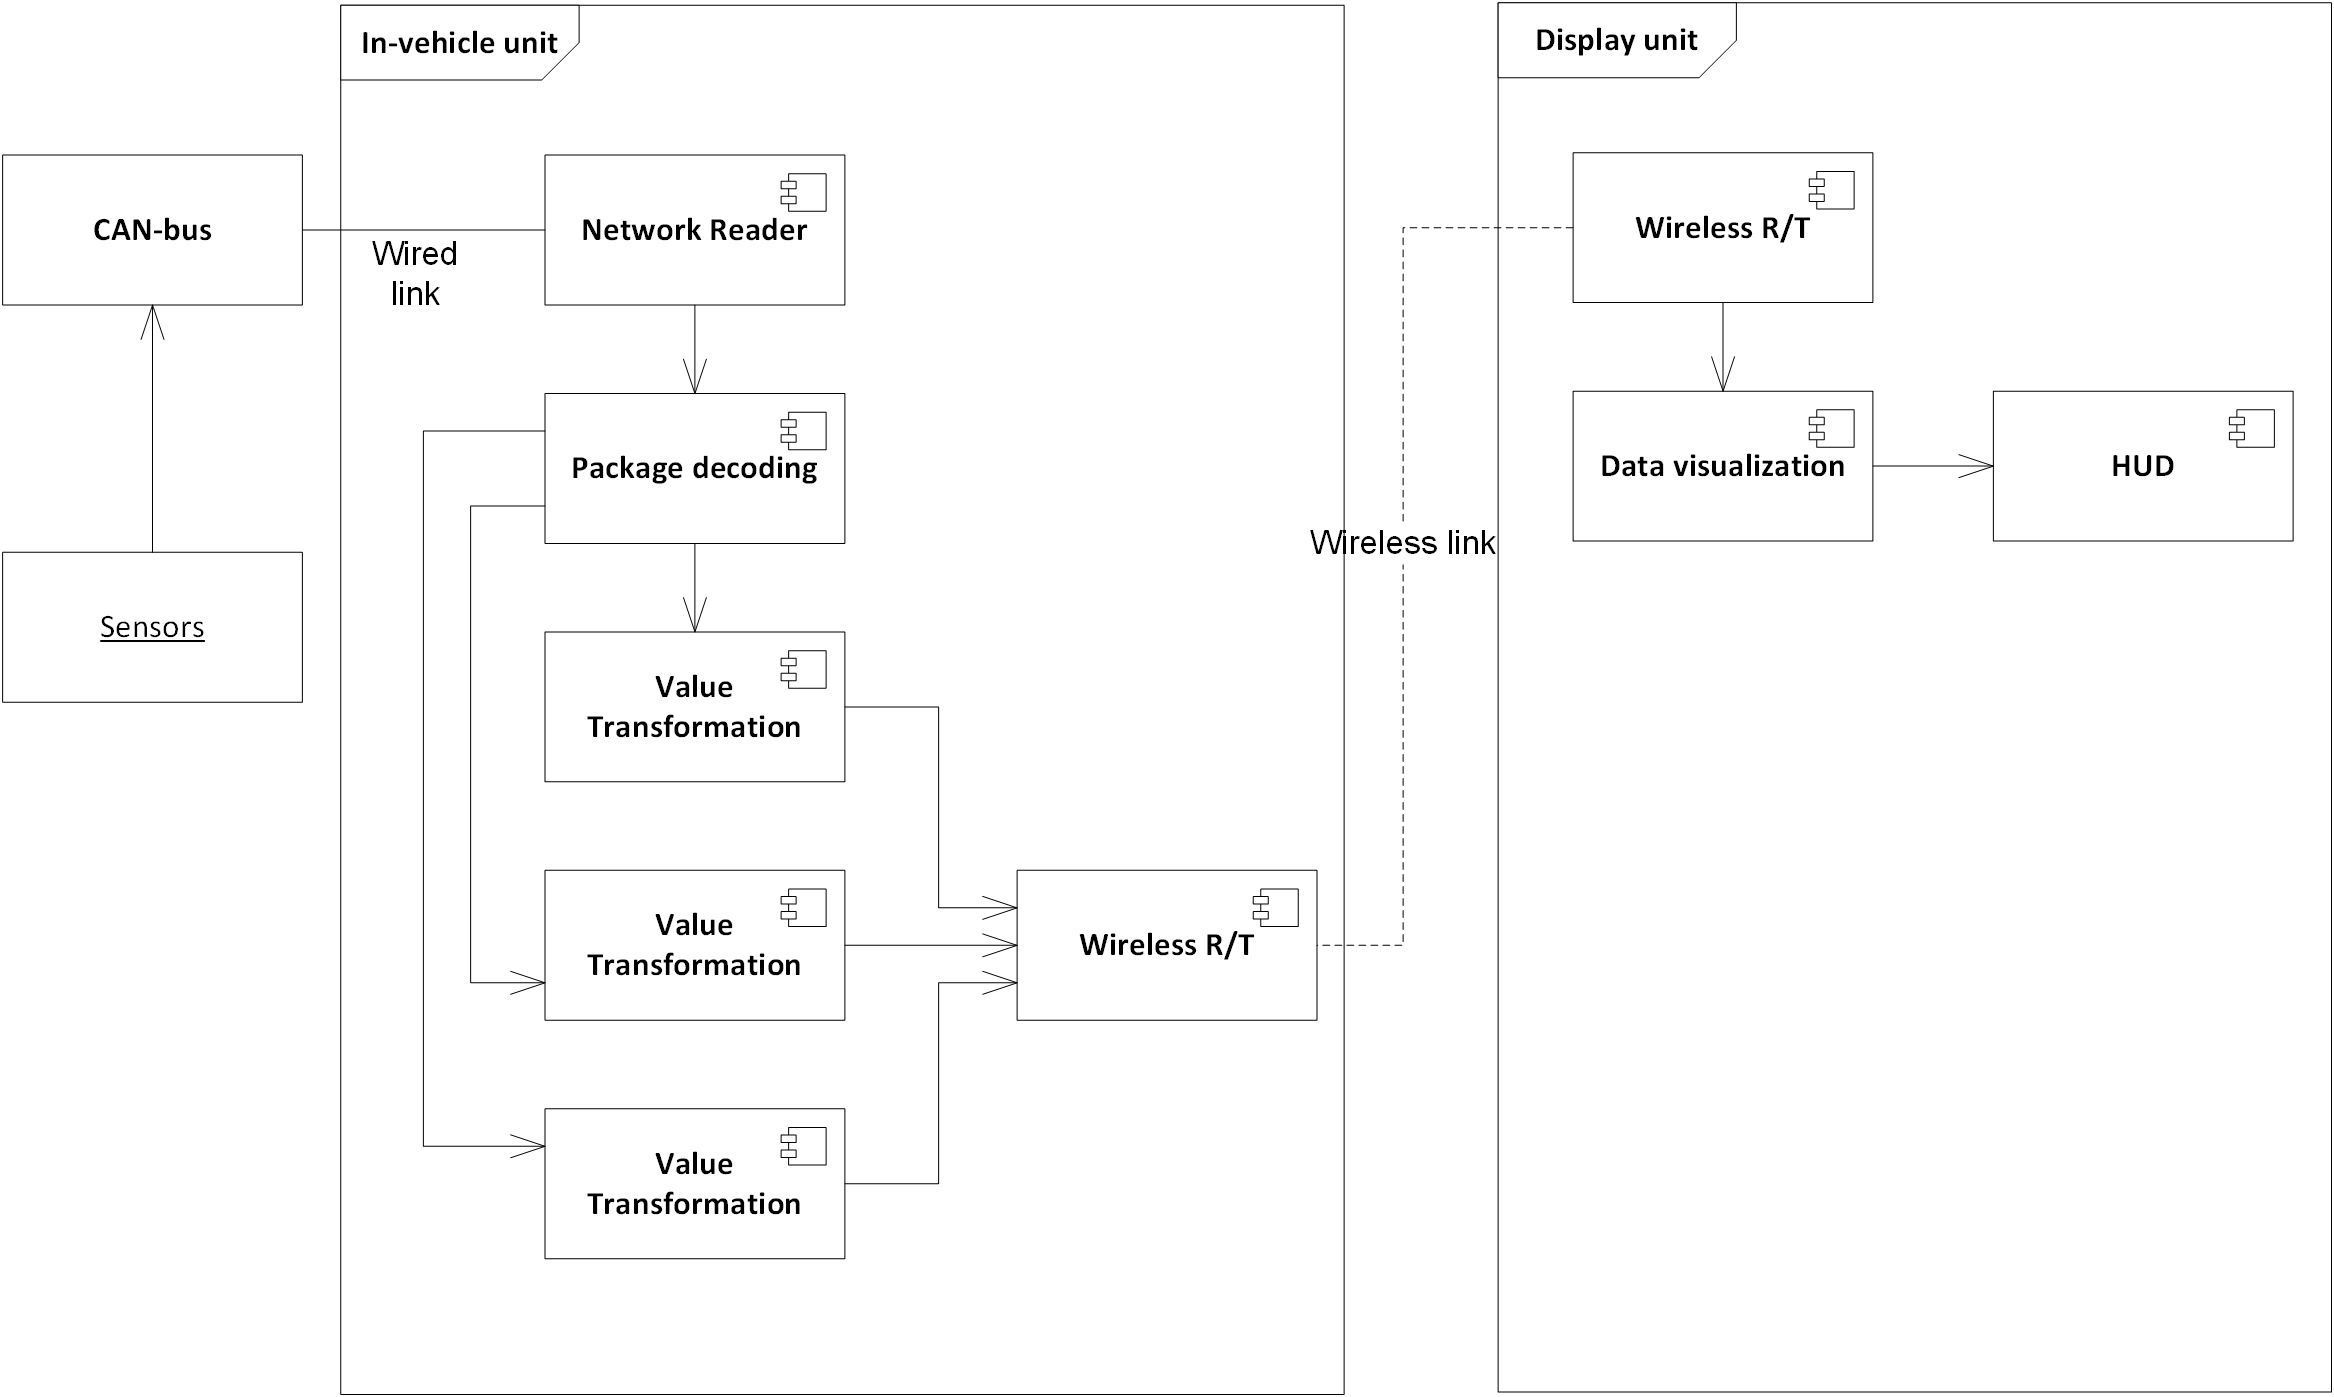
\includegraphics[width=\textwidth]{hw-sw-value-chain.png}
	\caption{Block diagram showing a simplified distribution of software
	components on the two computing nodes communicating wirelessly}
	\label{fig:hw-sw-value-chain}
\end{figure}

To be able to support rapid configuration of display layouts our system will
rely on a helper system with a design interface to generate a configuration
file that can be uploaded to the driver information system. The tool will load 
the sensor configuration profile to only show suitable display widgets for each sensor. The 
exchange format will be JSON due to very low overhead, and JSON being very
easy to support on different
systems. The format of the configuration file has yet to be specified, and will
to some extent be hardware dependent.

Sensor calibration profiles will be configured through configuration files of a
yet to be specified format, but JSON is also here a strong candidate. The idea
is to implement the transformation from uncalibrated to calibrated data via
reconfigurable filters in a pipe and filter pattern configured from the
calibration configuration file and uploaded to the DIS. The format also
specifies the output data format. 

\begin{figure}[!htbp]
	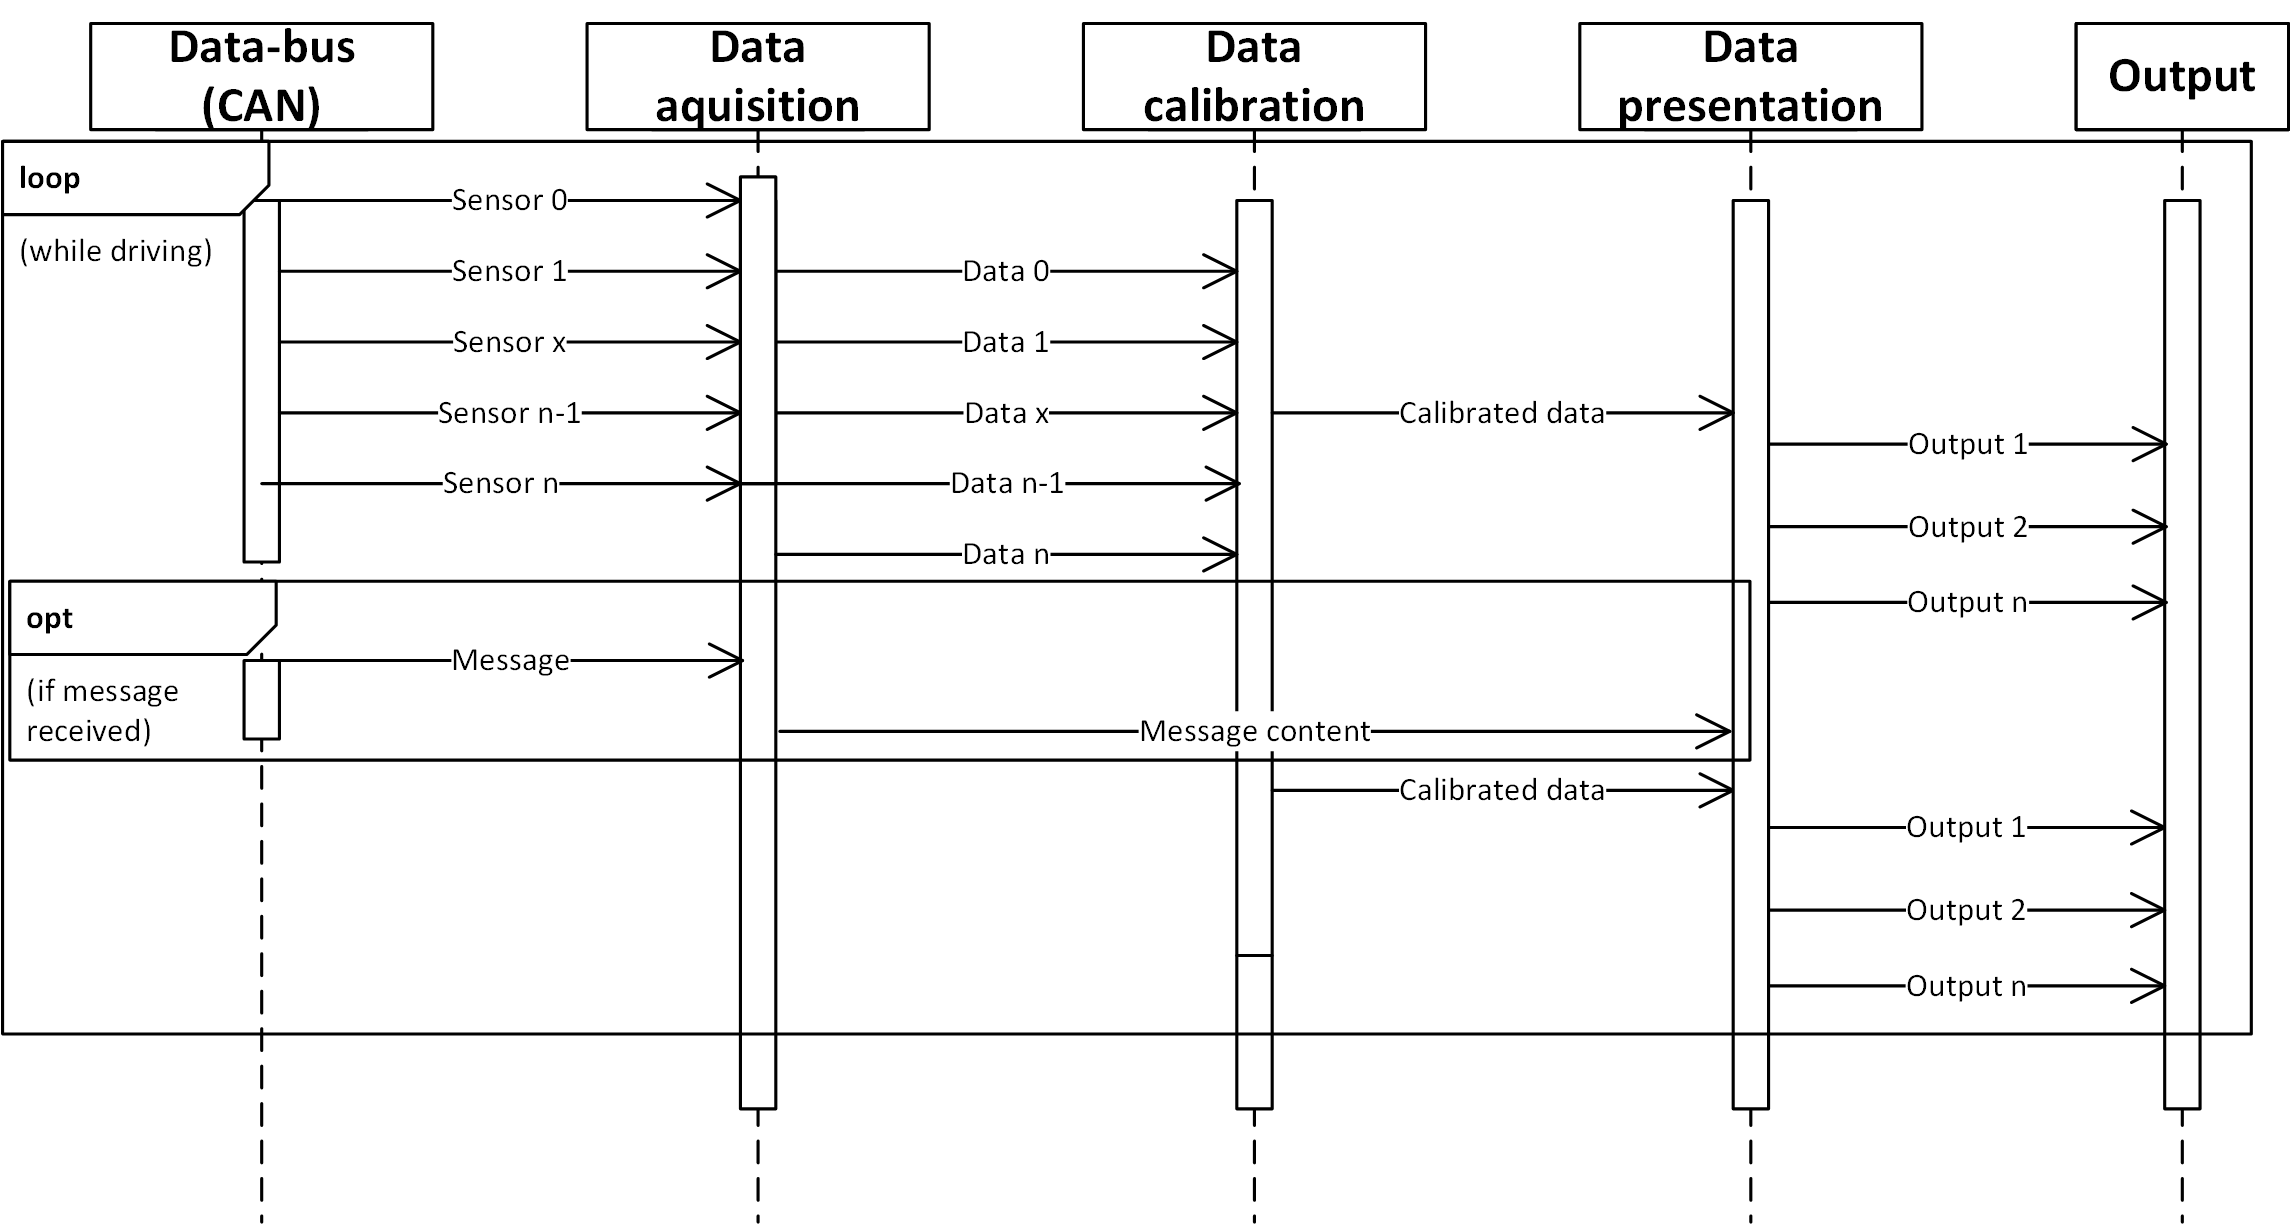
\includegraphics[width=\textwidth]{Basic_sequence_diagram.png}
	\caption{Asynchronous piping of data from input (left) to display output
	(right)}
	\label{fig:basic_sequence}
\end{figure}

Sensor profiles and package data format will also be configured via
configuration files that are uploaded to the DIS. The idea is to specify the
package formats and what type of data each sensor sends. Some sensors will send
an 8-bit integer value, while some may send 32-bit floating point numbers.
Using a layered approach to building the network control system allows the
system to load the package format at run-time. 

\vref{fig:basic_sequence} shows the basic sequence flow through the system, but
it also shows the system receiving and displaying a message. The feature is in
the requirements, but hasn't influenced the system architecture noteworthy. It
is however worth mentioning. The idea is that support crew can send messages to
the driver with the help of a computer interface and a radio-link with the
vehicle or DIS.

\begin{figure}[!htbp]
	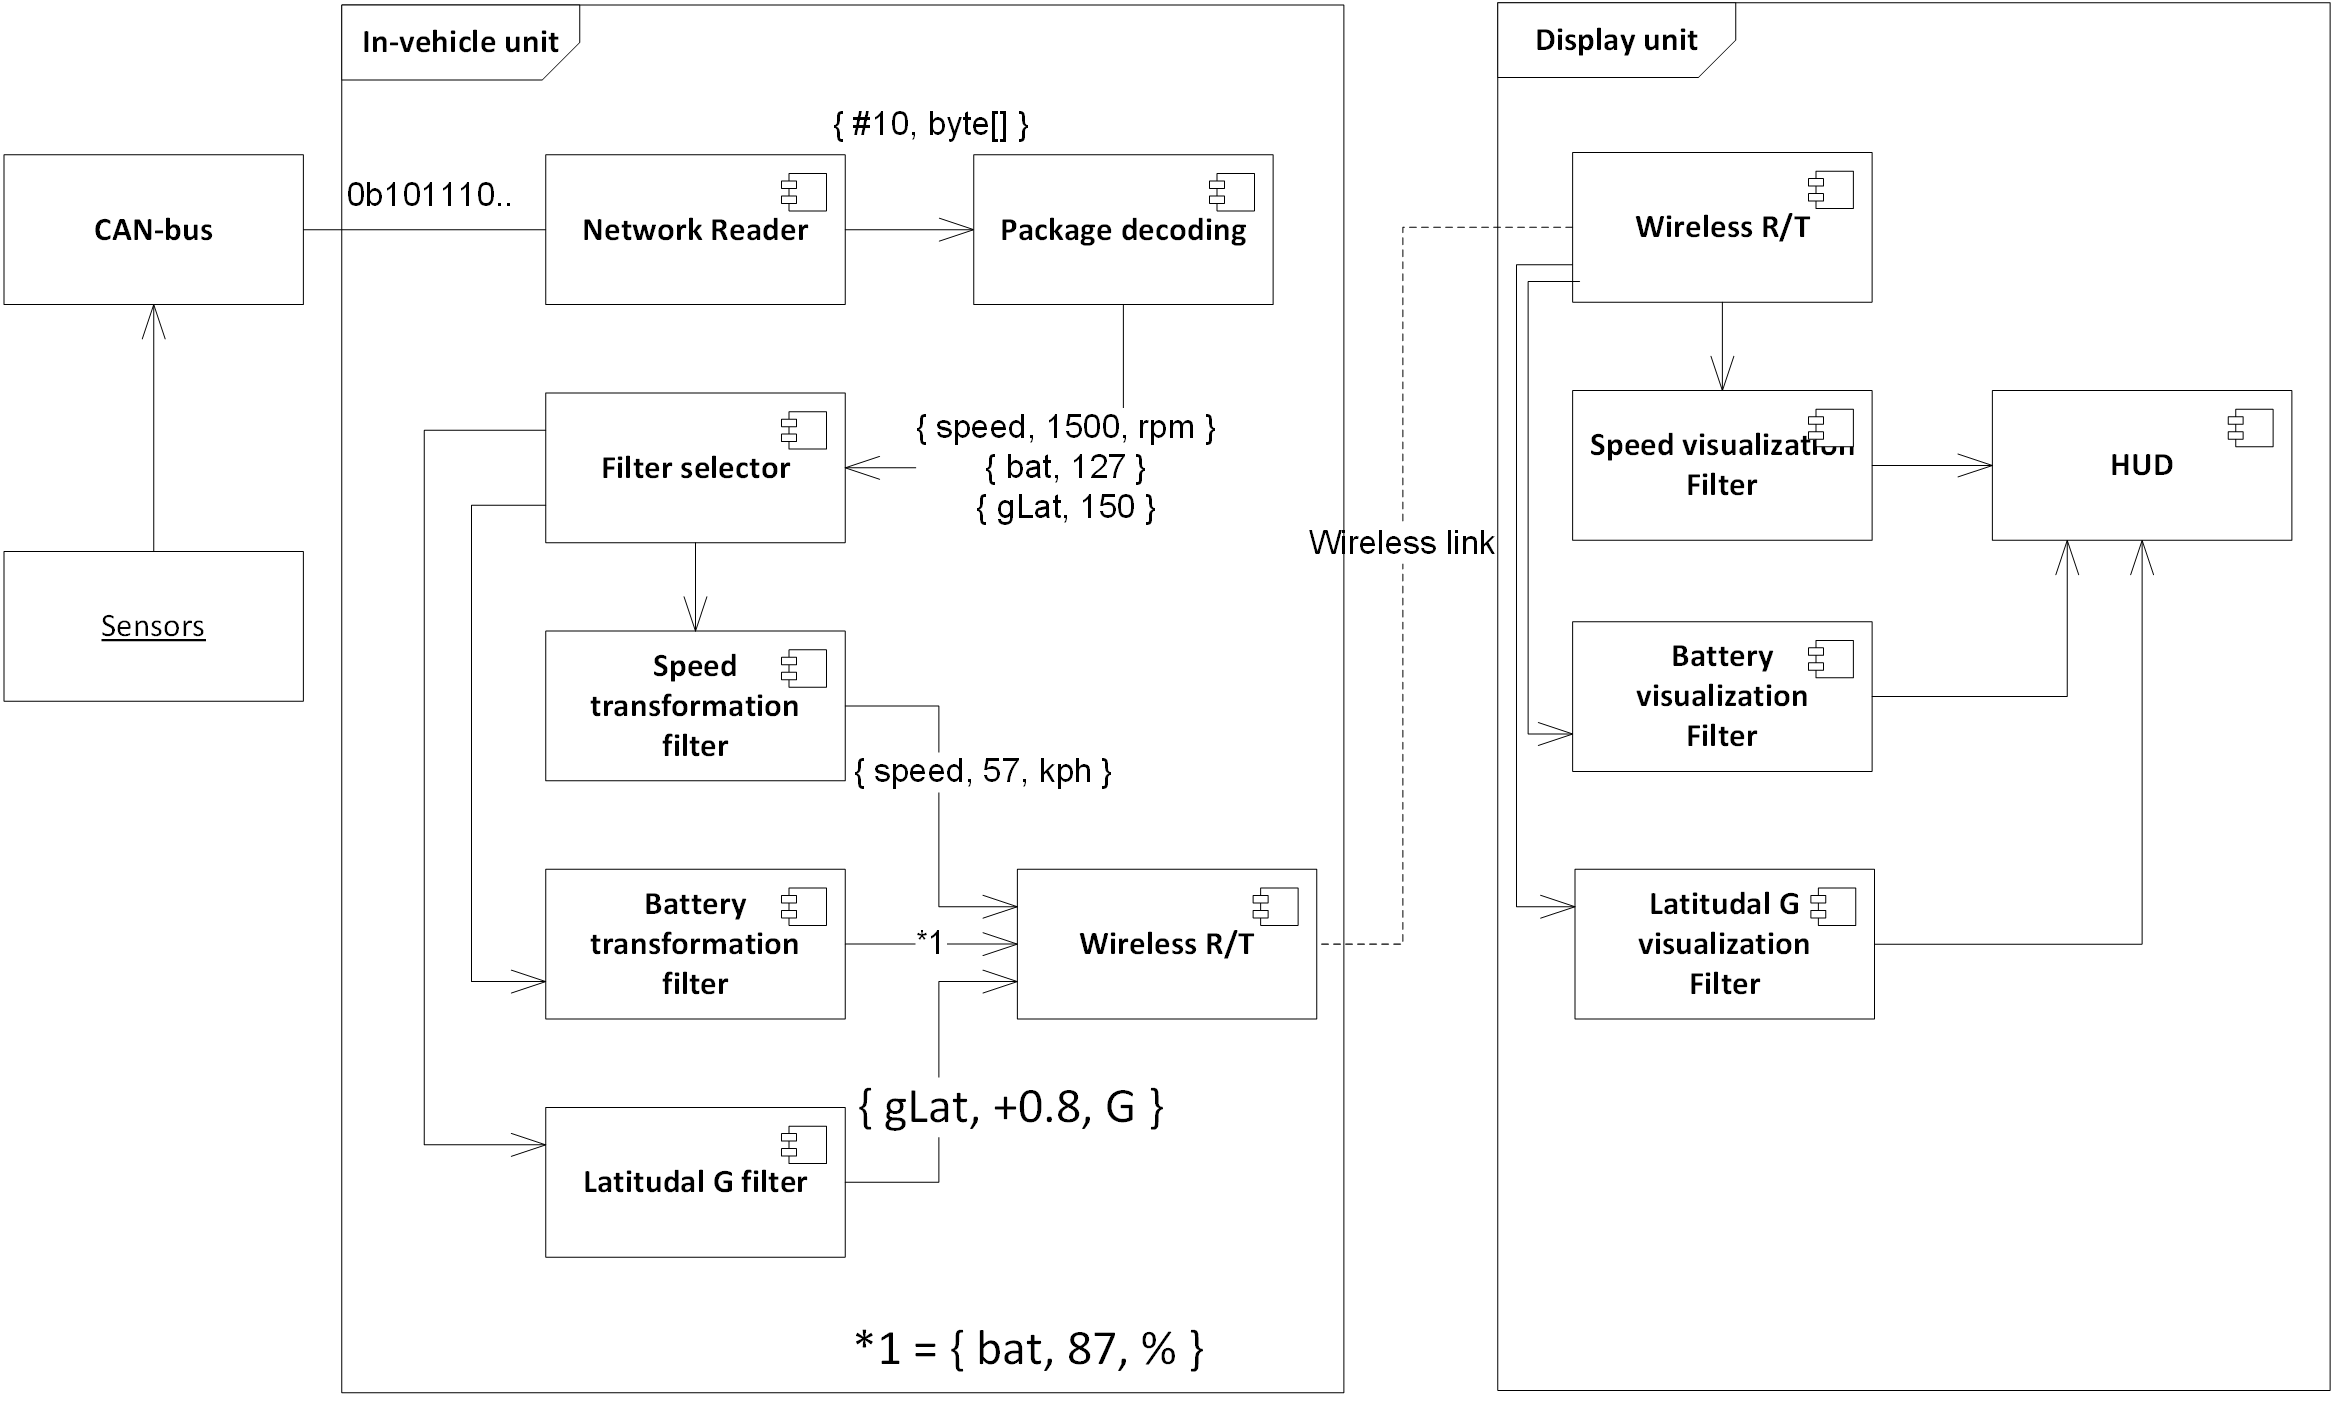
\includegraphics[width=\textwidth]{hw-sw-value-chain-with-example-values.png}
	\caption{Example of a possible configuration of the DIS showing the conversion
	of data between formats and from sensor value to the real world values
	actually measured by the sensor. 
	}
	\label{fig:hw-sw-value-chain-examples}
\end{figure}

The domain layer model describes the driver information system architecture,
and comparing \ref{fig:hw-sw-value-chain-examples} and \ref{fig:domain-layer-model}
shows how closely the high-level software architecture resembles the
domain-layer. 

\begin{figure}[!htbp]
	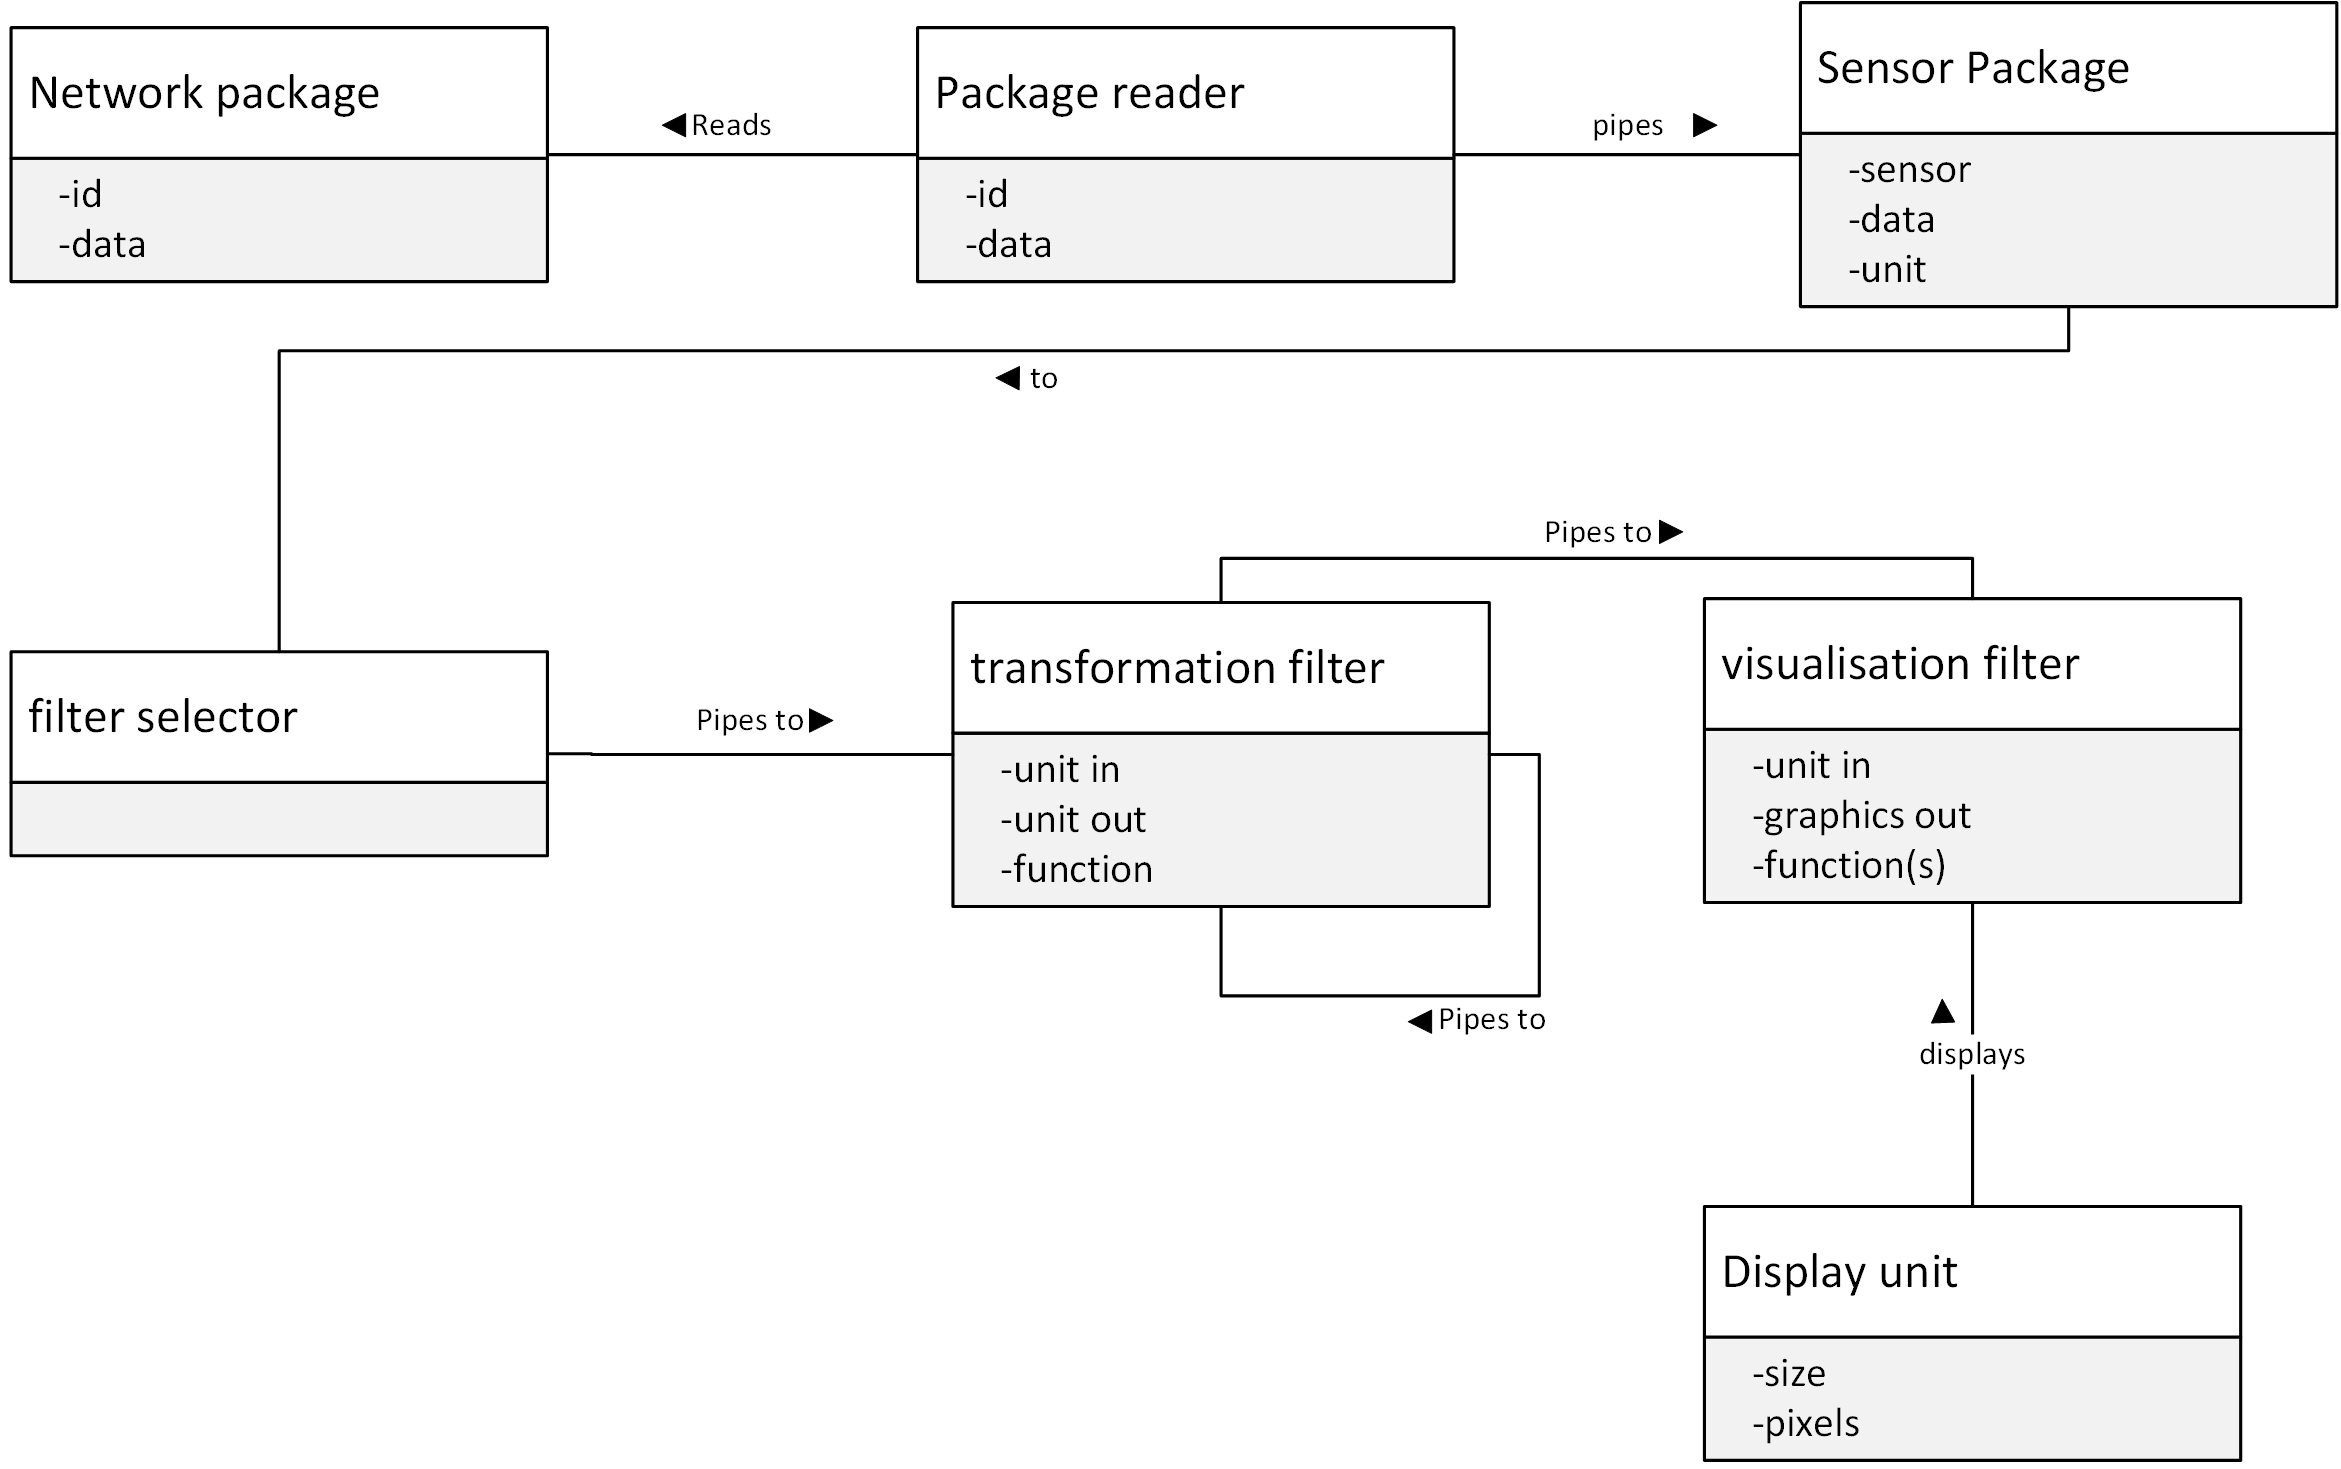
\includegraphics[width=\textwidth]{domain-layer-model.png}
	\caption{Domain layer model showing the connections between different system
	components and their relationship.
	}
	\label{fig:domain-layer-model}
\end{figure}

\section{Proof-of-concept configuration tool for display layout}
\label{results:poc}
During this project we have prototyped a GUI-tool for configuring the display
layout of the HUD. We used the proof-of-concept (PoC) to evaluate our ideas of
the design of the GUI-tool and to evaluate its functionality. Our conclusion
was that the design was well suited for the purpose and that a fully functional
implementation of this tool would be a close to ideal way of rapidly
configuring a display layout, and thus helping to meet the system requirements.
With the PoC system we were able to mock up layouts in less than 1 minute. The
prototype was created with Qt 5 \cite{qt:digiaAboutUs}.

\begin{figure}[!htbp]
	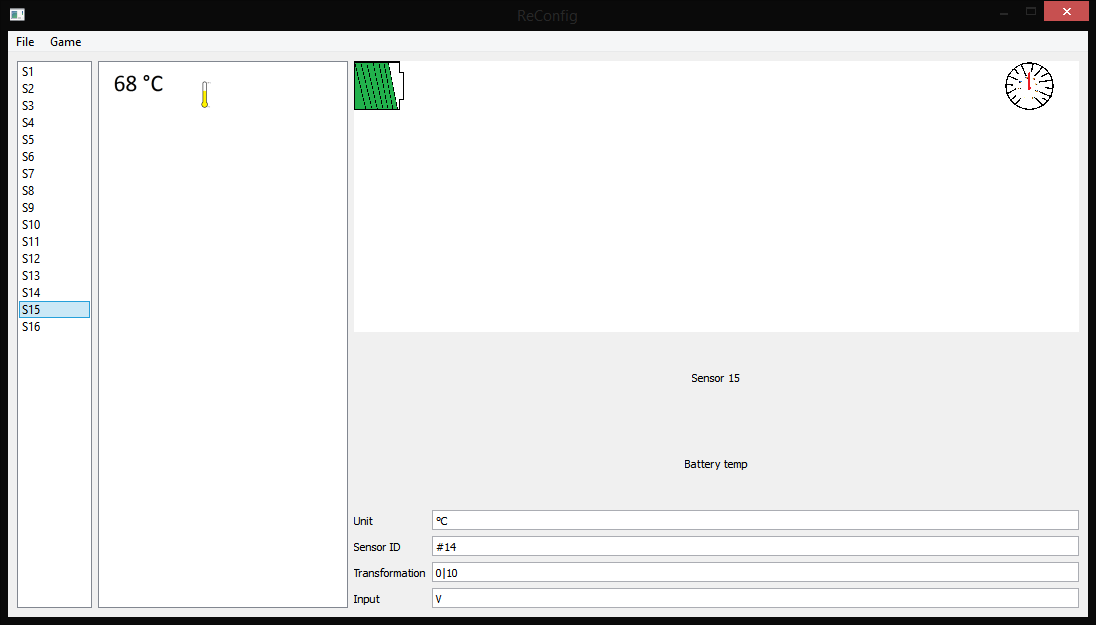
\includegraphics[width=\textwidth]{revision-poc-screenshot.PNG}
	\caption{Screenshot of our PoC layout tool. The layout of the screen is
	shown in the upper right corner, while sensor data is shown below. The left
	pane shows the list of sensors loaded, and the middle pane shows available
	widgets for the currently selected sensor.
	}
	\label{fig:poc-screenshot}
\end{figure}

\section{Verification of design}
Since the system described herein has not been developed we have not had any
chance to verify our design. We do, however, propose a set of metrics that can
be used to verify the architecture. They include measuring latency of the DIS, 
measuring time spent on creating configurations,
and measuring driver response when compared to a traditional HDD system. We
also suggest that feedback from the drivers can be used both for verification and
further development, but that is outside the scope of this project. For all
measures and metrics we refer to appendix \vref{appendix:sad}. 
